\begin{exercise}
    Sei $A := \Bbraces{a_1, a_2}$ und $B := \Bbraces{b_1, b_2, b_3}$ zwei Trägermengen und gemeinsam mit den zyklischen Permutationen $f_A: a_1 \mapsto a_2 \mapsto a_1$ und $f_B: b_1 \mapsto b_2 \mapsto b_3 \mapsto b_1$ zwei Algebren. Zeigen Sie, dass es auf dem direkten Produkt $(C, f_C)$ der beiden keine Unteralgebra gibt, die eine isomorphe Kopie einer der ursprünglichen Algebren ist.
\end{exercise}

\begin{solution}
    Zwei mögliche Unteralgebren sind natürlich die trivialen, also einmal die ganze Algebra $(C, f_C)$ und die leere Menge. Beide sind allerdings weder zu $(A, f_A)$ noch zu $(B, f_B)$ isomorph. Betrachten wir also eine Trägermenge $D \subseteq C$ mit $D \neq \emptyset$ und $D \neq C$. Das heißt es gibt ein $i \in \Bbraces{1, 2}$ und ein $j \in \Bbraces{1, 2, 3}$ mit $(a_i, b_j) \in D$. Wählen wir nun  $k \in \Bbraces{1, 2}$ und $l \in \Bbraces{1, 2, 3}$ so ,dass $(a_l, b_k) \notin C$. Durch mehrmaliges anwenden von $f_C$ auf $(a_i, b_j)$ erhält man $(a_l, b_k)$ also kann $(D, f_C)$ keine Unteralgebra von $(C, f_C)$ sein.
    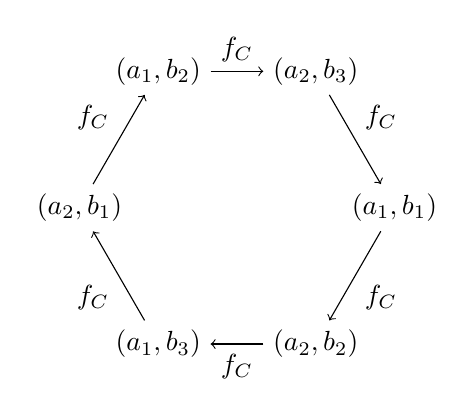
\begin{tikzpicture}[auto]
        \node (1) at (0:2) {$(a_1, b_1)$};
        \node (2) at (300:2) {$(a_2, b_2)$};
        \node (3) at (240:2) {$(a_1, b_3)$};
        \node (4) at (180:2) {$(a_2, b_1)$};
        \node (5) at (120:2) {$(a_1, b_2)$};
        \node (6) at (60:2) {$(a_2, b_3)$};

        \draw[->] (1) to node {$f_C$} (2); 
        \draw[->] (2) to node {$f_C$} (3); 
        \draw[->] (3) to node {$f_C$} (4); 
        \draw[->] (4) to node {$f_C$} (5); 
        \draw[->] (5) to node {$f_C$} (6); 
        \draw[->] (6) to node {$f_C$} (1); 
    \end{tikzpicture}
    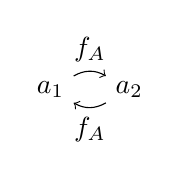
\begin{tikzpicture}[auto, bend left]
        \node (1) at (0,0) {$a_1$};
        \node (2) at (1,0) {$a_2$};

        \draw[->] (1) to node {$f_A$} (2);
        \draw[->] (2) to node {$f_A$} (1);
    \end{tikzpicture}
    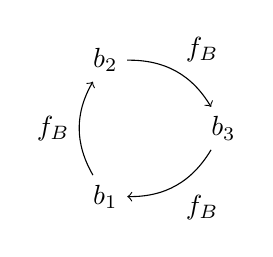
\begin{tikzpicture}[auto, bend left]
        \node (1) at (0:1) {$b_3$};
        \node (2) at (120:1) {$b_2$};
        \node (3) at (240:1) {$b_1$}; 

        \draw[->] (3) to node {$f_B$} (2);
        \draw[->] (2) to node {$f_B$} (1);
        \draw[->] (1) to node {$f_B$} (3);
    \end{tikzpicture}
\end{solution}